%%%%%%%%%%%%%%%%%%%%%%%%%%%%%%%%%%%%%%%%%
% University/School Laboratory Report
% LaTeX Template
% Version 3.1 (25/3/14)
%
% This template has been downloaded from:
% http://www.LaTeXTemplates.com
%
% Original author:
% Linux and Unix Users Group at Virginia Tech Wiki 
% (https://vtluug.org/wiki/Example_LaTeX_chem_lab_report)
%
% License:
% CC BY-NC-SA 3.0 (http://creativecommons.org/licenses/by-nc-sa/3.0/)
%
%%%%%%%%%%%%%%%%%%%%%%%%%%%%%%%%%%%%%%%%%

%----------------------------------------------------------------------------------------
%	PACKAGES AND DOCUMENT CONFIGURATIONS
%----------------------------------------------------------------------------------------

\documentclass[UTF8]{ctexart}

\usepackage{siunitx} % Provides the \SI{}{} and \si{} command for typesetting SI units
\usepackage{graphicx} % Required for the inclusion of images
\usepackage{graphics} % 图片设置
\usepackage{subfigure} 

\usepackage{natbib} % Required to change bibliography style to APA
\usepackage{amsmath} % Required for some math elements 
\usepackage{amssymb} % 使用因为所以符号
\usepackage{fancyhdr} % 使用页眉

\usepackage{algorithm}
\usepackage{algorithmic}

\usepackage{listings} % 插入代码
\usepackage{xcolor}

\usepackage{enumerate} % 列表

\lstset{
    %backgroundcolor=\color{red!50!green!50!blue!50},%代码块背景色为浅灰色
    rulesepcolor= \color{gray}, %代码块边框颜色
    breaklines=true,  %代码过长则换行
    numbers=left, %行号在左侧显示
    numberstyle= \small,%行号字体
    %keywordstyle= \color{red},%关键字颜色
    commentstyle=\color{gray}, %注释颜色
    frame=shadowbox%用方框框住代码块
    }

%\usepackage{url} % 引用URL
% \usepackage{cite}
% \newcommand{\upcite}[1]{\textsuperscript{\textsuperscript{\cite{#1}}}} %参考文献上标
%\bibliographystyle{plain}   %引用的样式%

\pagestyle{fancy}
\fancyhf{} 
\cfoot{\thepage} 

\setlength\parindent{0pt} % Removes all indentation from paragraphs

\renewcommand{\labelenumi}{\alph{enumi}.} 

%----------------------------------------------------------------------------------------
%	DOCUMENT INFORMATION
%----------------------------------------------------------------------------------------
\title{算法分析与设计-作业十}

\author{王宸昊 2019214541}

\date{\today}

\begin{document}

\maketitle

%----------------------------------------------------------------------------------------
%	SECTION 1
%----------------------------------------------------------------------------------------

\section{CLRS, Page,594 32.4-8}

实现的算法如下:

\begin{lstlisting}[mathescape]
    m=P.length
    $\pi$=COMPUTE-PREFIX-FUNCTION(P)
    for q=0 to m
      for each character a in $\Sigma$
        if P[q+1]==a
          $\delta$(q,a)=q+1
        else if q==m or P[q+1]!=a
          $\delta$(q,a)=$\delta$($\pi$[q],a)
    return $\delta$
\end{lstlisting}

证明:由定义可知,设$\sigma (x)=max\{k;P_k \sqsupset x\}$,若$q=m$或$P[q+1]\neq a$则$\delta(q,a)=\sigma (P_q a),\delta(\pi[q],a)=\sigma (P_{\pi[q]} a)$。对于$P_q$本身,有$\sigma(P_q)=\pi[q]$。所以对$P_q$长度为$\pi[q]$的后缀串$s$,同时也是$P_q$相同长度的前缀。所以有$\delta(q,a)=\delta(\pi[q],a)$.


%----------------------------------------------------------------------------------------
%	SECTION 2
%----------------------------------------------------------------------------------------

\section{CLRS, Page, 594 32-1}

\subsection{a.设计有效的算法,分析运行时间}

对字符串$P_i$,使用KMP算法的 \textbf{COMPUTE-PREFIX-FUNCTION(P)} 求得$\pi[i]$。计算$k=i-\pi[i]$,若$i$可以整除$k$,则$r=i/k$,否则$r=1$。

所花时间为$O(m)$。

\subsection{b.证明期望为O(1)}

假设$i=w$时使得$r=\rho (P_i)$最大,那么最小元字符串长度可表示为$k=w/r$。出现这样的二进制字符串的概率为:
$$P_w=\frac{1}{2^{k*(r-1)}}=\frac{1}{2^{w*\frac{r-1}{r}}}$$
那么总体概率
$$P=\Sigma_{w=1}^{m}\frac{1}{2^{w*\frac{r-1}{r}}}<=\Sigma_{w=1}^{m}\frac{1}{2^{w*r}}<=\frac{1}{2^r}\Sigma_{w=1}^{m}\frac{1}{w}=O(1)$$

\subsection{c.证明算法正确性}

由定义可知,$k$是模式$P$的最大重复因子,那么当$T[s+q+1]!=P[q+1]$时,跳过所有的重复子串,即跳过$\lceil q/k\rceil$,再进行比较,依然是正确的。\\

复杂度:均摊分析可知,$s$只在12行被增加,最多增加$n-m$次,所以大循环最多执行$n-m$次;$q$只在第8行被增加,最多增加到$k*\rho^{*}(P)$;而q在第13行被减为0,所以$q=q+1$最多执行了$(n-m)*k*\rho^{*}(P)$,即算法复杂度为$O(\rho^{*}(P)*n+m)$


%----------------------------------------------------------------------------------------
%	SECTION 3
%----------------------------------------------------------------------------------------
\section{CLRS, Page, 447 26-2}

\subsection{实验环境:}

编译环境为C++10,操作系统的版本为Windows 10。GUI框架选用QT5\\
硬件环境为:CPU为AMD Ryzen 7 1700(3.0 GHz),RAM 16G。

\subsection{实验运行:}

可执行EXE文件位于exe目录下,已设置自解压,右键执行exe,解压到当前目录下,自动运行。\\

编译源码请使用Qt Creator打开.pro文件,在Qt Creator中编译执行。

\subsection{实验原理:}

\subsubsection{Brute-Force算法}

将匹配串和模式串左端对齐,依次跟模式串的每一位比较是否一致,如果不一致将匹配串右移一位。将匹配中的首位位置记录下来。\\

同时暴力法不需要预处理。。假设匹配串的长度为m, 模式串的长度为n, 则算法的复杂度为$O(mn)$。

\subsubsection{KMP算法}

KMP算法的基本思想是主串不回溯,通过计算前缀数组,每次不匹配时,不需要每次回退主串的下标,而且通过前缀数组记录的信息进行重新对齐。\\

预处理操作包括$O(n)$计算前缀数组,同时还需要$O(n)$的空间,算法的复杂度为$O(m)$


\subsubsection{BM算法}

BM算法的思想是如果在模式串中不存在的字符,那么肯定不会满足匹配的情况,这样可以通过辅助数组向后多移动几位。\\

根据好后缀和坏字符规则向后滑动的位数,取大的,作为滑动次数。\\

匹配的时间复杂度为$O(m)$

\subsection{实验结果:}

测试数据集共设计了两种。位于data目录下。\\

数据集1是原版的哈利波特的TXT文件,每个文件包含几十万个英文数字字符和标点符号。\\
数据集2是Python脚本随机生成的字符文本,字符集合包括英文字母数字和特殊符号,数据集大小在两百万。\\

程序的界面设计和运行效果如图\ref{result1}:

\begin{figure}[H]
    \centering
    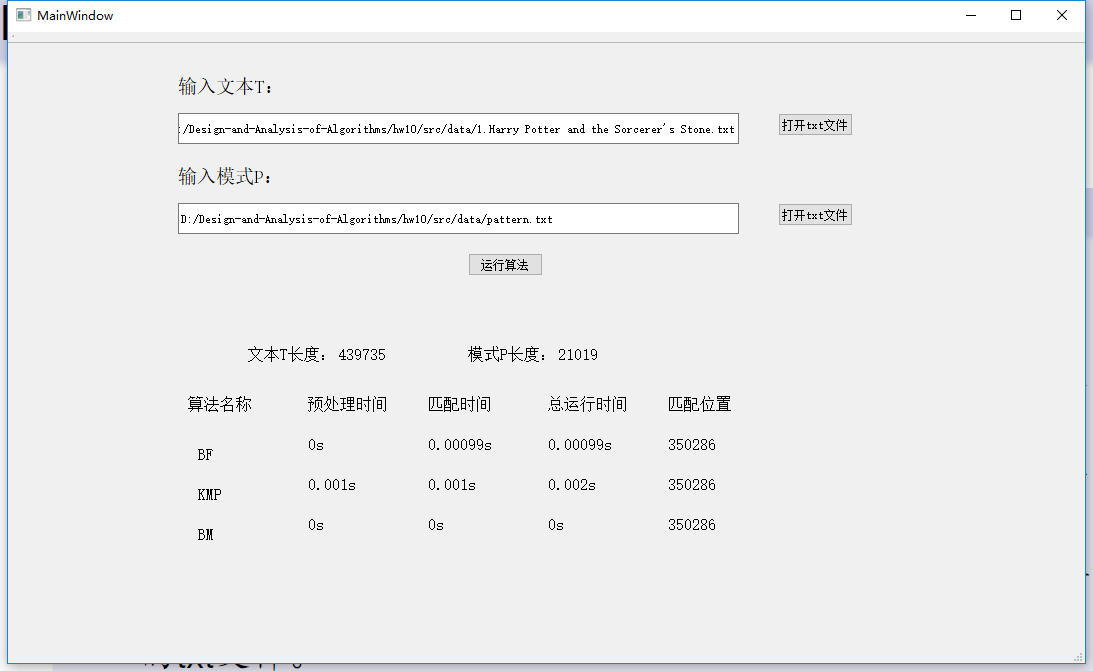
\includegraphics[width=1\textwidth]{img/result1.png}
    \caption{实验一运行效果}
    \label{result1}
\end{figure}

下面做了两组实验,第一组实验的数据是哈里波特小说的第一部,包含439735个字符,模式串的长度为21019。\\
实验二是随机生成的字符串,文本的长度为200 0005, 模式串的长度为324676。

\begin{figure}[H]
    \centering
    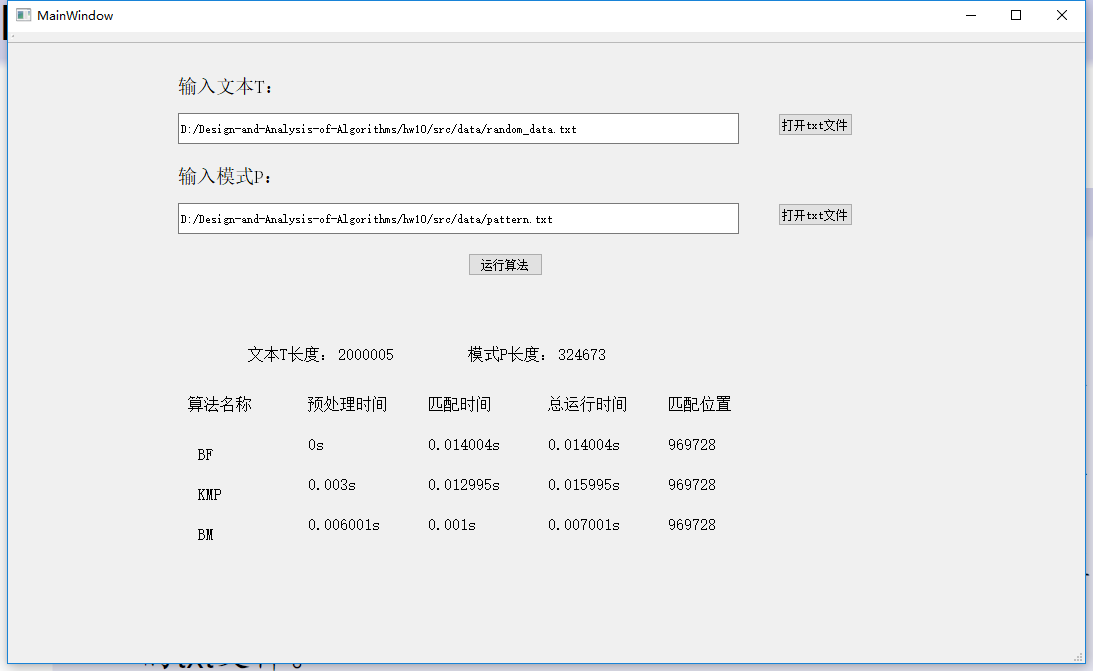
\includegraphics[width=1\textwidth]{img/result2.png}
    \caption{实验二运行效果}
    \label{result2}
\end{figure}

图\ref{result1}和图\ref{result2}是实验效果,实验总运行时间的对比如下:

\begin{table}[H]
    \caption{字符串匹配算法性能测试}
    \label{table-1}
    \begin{center}
        \begin{tabular}{ccc}
            \hline
            算法&       实验一执行时间(s) &     实验二执行时间(s)\\     
            \hline
            BF&         0.00099 &           0.014004  \\  
            KMP&        0.002 &             0.015995  \\ 
            BM&         0 &                 0.007001  \\                     
            \hline
        \end{tabular}  
    \end{center}
\end{table}

从实验结果上看可以看出,BM算法的性能要优于其他两种算法不少,KMP算法略优于暴力算法,但是在极端情况下,算法的性能会出现退化。

\end{document}
